\section{\emph{Wireless Power Transmission}}

Como o próprio nome já induz, essa tecnologia faz referência a uma forma eficiente de transferir energia elétrica sem o uso de qualquer substância ou fio. O intuito dela é ser usada em locais inacessíveis ou inconvenientes para utilização de outros meios físicos. Dentro dessa tecnologia, os meios mais comuns para fazer a transmissão de energia são o laser, ondas milimétricas ou micro-ondas.

Historicamente falando, essa tecnologia vem tentando ser aplicada desde 1897 quando Nikola Tesla deu início ao seu experimento com a \emph{``World Wireless''}, que mais tarde foi patenteada como \emph{``World Wireless System''}. O Primeiro eventual sucesso com a tecnologia \emph{Wireless Power Transmission} (WPT) só se deu em 1963 através da \emph{Raytheon Company}.

Quanto ao desenvolvimento do WPT, partindo do princípio de Lavoisier (1743-1794) “Na Natureza, nada se cria, nada se perde, tudo se transforma”, o primeiro passo é entender que a energia deve estar tratada de uma forma adequada para viajar pelo ar e, posteriormente, entender que isso nos levará ao desenvolvimento de um sistema para transmissão e recepção compatíveis para essa energia.

Com foco maior no nosso projeto, dentro dessa tecnologia, optamos por trabalhar com o modelo LPT, ou seja, uma transmissão via laser, que é um dos meios de transmissão direta, onde é necessário possuir visada entre o transmissor e receptor, o que limitará a distância de aplicação, mas não a eficiência. Iremos discutir a frente o desenvolvimento desse modelo.

\subsection{DLC - \emph{Distributed Laser Charging}}

O que diferencia o módulo DLC com os outros tipos de carregadores LPT é o sistema retrorrefletor que possibilita a segurança na transmissão de energia.

Utilizado em sinais de trânsito, bicicleta e automóveis, os retrorrefletores são “[...]sistemas ópticos que possuem a notável propriedade de, recebendo um raio luminoso, fazer com que ele retorne em uma direção paralela à de incidência com um mínimo de deslocamento.” [22]. Portanto, seu princípio de funcionamento engloba a Lei de Reflexão e a Lei da Refração.

No espelho de tela plana, a luz refletida é paralela a sua luz incidente somente quando o ângulo de incidência for vertical em relação ao espelho. Porém, no dispositivo, há três espelhos dispostos que, perpendicularmente, formam o retrorrefletor independentemente do seu ângulo de incidência, como mostra a figura \ref{retroreflector_cubo}.

\begin{figure}[ht!]
	\centering
	\caption{Retrorrefletor}
	\label{fig:retroreflector_cubo}
	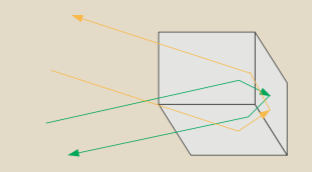
\includegraphics{retroreflector_cubo}[scale=1]
	\smallcaption{Fonte: ZHANG, FANGM KIU, WU, XIA, YANG: Distributed Laser Charging: A Wireless Power Transfer Appoach. IEEE Internet of Things journal, vol 5, no 5, pp 3853-3864, 2018. Disponível em: \url{https://ieeexplore.ieee.org/document/8398229/}. Acesso: 07 junho 2021.}
\end{figure}

DLC é uma tecnologia de \emph{Wireless Power Transfer} baseada em Lasers ressonantes e distribuídos. Os componentes óticos são divididos em duas partes, transmissor e receptor, respectivamente. 

A Figura 11 mostra o diagrama do sistema DLC. Um espelho retrorrefletor R1 com uma refletância de 100\% e um ganho médio estão presentes no transmissor. No receptor há um espelho R2 retrorrefletor com uma refletância parcial de 95\%. Os espelhos R1, R2 e o ganho médio formam a cavidade ressonante, onde os fótons são amplificados formando um laser ressonante de cavidade interna. Os fótons capazes de passar pelo espelho R2 formam o laser de cavidade externa. Este pode ser convertido em eletricidade através de uma célula fotovoltaica instalada atrás do espelho R2.

\begin{figure}[ht!]
	\centering
	\caption{Diagrama do sistema DLC}
	\label{fig:dlc}
	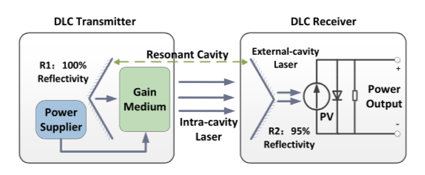
\includegraphics{dlc}[scale=1]
	\smallcaption{Fonte: ZHANG, FANGM KIU, WU, XIA, YANG: Distributed Laser Charging: A Wireless Power Transfer Appoach. IEEE Internet of Things journal, vol 5, no 5, pp 3853-3864, 2018. Disponível em: \url{https://ieeexplore.ieee.org/document/8398229/}. Acesso: 07 junho 2021.}
\end{figure}

No sistema DLC, fótons são amplificados sem a preocupação de seus ângulos de incidência, contanto que eles viajem dentro da linha de visão dos espelhos R1 e R2. Por isso, o laser de cavidade interna gerado pelo ressonador pode se auto alinhar sem um posicionamento ou rastreamento. Essa característica possibilita que usuários carreguem seus dispositivos sem um posicionamento cauteloso do mesmo. O Sistema DLC é intrinsecamente seguro, pois caso um objeto esteja bloqueando a linha de visão do laser de cavidade interna, o objeto pode parar o laser imediatamente, cancelando a ressonância. Essas características oferecem ao sistema DLC a capacidade de carregar dispositivos a longa distância.



\subsection{Dispositivos LPT disponíveis}

\subsubsection{PowerLight Technologies}

A \emph{PowerLight Technologies} é uma empresa americana de engenharia de transmissão de energia LPT que surgiu em 2006 com o nome de \emph{LaserMotive} para concorrer na \emph{Power Beam Challenge}, que faz parte da \emph{Centennial Challenges da NASA}. Após vencer o concurso de 2009, a empresa foca no desenvolvimento da tecnologia para alimentar VANTs (Veículo Aéreo Não Tripulado) e atua em parceria com a NASA para criar uma arquitetura que permite utilizar lasers para o lançamento de foguetes e satélites. [23].

\subparagraph{PowerLight Free-Space Power Beaming}

Em junho de 2012, a \emph{LaserMotive} conseguiu alimentar um \emph{Stalker Unmanned Aerial System} (UAS) da \emph{Lockheed Martin} por mais de 48 horas, sendo considerado um recorde na época [23].

\subsubsection{PTROL (Power Transmitted Over Laser) Project}

Em maio de 2019, a \emph{PowerLight} transmitiu 400 watts via laser a uma distância de 325 metros. O receptor converte a energia do laser em DC passando por um inversor que alimenta luzes, laptops e uma cafeteira.

As células fotovoltaicas no receptor foram modificadas para conseguir uma melhor resposta em um comprimento de onda e, também, no equipamento constava um sistema de segurança que interrompia a transmissão em qualquer obstáculo colocado entre o emissor e o receptor. [24]